%!TEX root = ../Thesis.tex
%Chapter 1

\chapter{Real Eigenvalues of complex potentials}
\label{ChapterRealEigenValues}
\lhead{ChapterRealEigenValues. \emph{Real Eigenvalues of complex potentials}} % Write in your own chapter title to set the page header
%
The complex eigenvalues of some non-Hermitian Hamiltonians, e.g. parity-time symmetric Hamiltonians, come in complex-conjugate pairs. We show that for non-Hermitian scattering Hamiltonians (of a structureless particle in one dimension) possesing one of four certain symmetries, the poles of the $S$-matrix eigenvalues in the complex  momentum plane are symmetric about the imaginary axis, i.e. they  are complex-conjugate pairs in complex-energy plane. This applies even to states which are not bounded eigenstates of the system, i.e. antibound or virtual states, resonances, and antiresonances. The four Hamiltonian symmetries are formulated as the commutation of the Hamiltonian with specific antilinear operators. Example potentials with such symmetries are constructed and their pole structures and scattering properties are calculated.
%
\newpage
%
%
\section{Introduction}
%
%
%
%
Non-Hermitian (NH) Hamiltonians may represent effective interactions for components of a system. Feshbach's partitioning technique \cite{Feshbach1958,Feshbach1962} provides the formal framework to find NH-Hamiltonians for a subspace, from the Hermitian Hamiltonian for the total system. NH-Hamiltonians are also set phenomenologically to mimic some observed or desired behaviour, such as gain, decay or absorption in nuclear or atomic, molecular, and optical physics \cite{Muga2004,Feng2017,El-Ganainy2018,Moiseyev2011,Longhi2017a,Konotop2016}. They arise as well as auxiliary tools to facilitate calculations of cross sections  or resonances, e.g. by complex scaling of the coordinates \cite{Aguilar1971,Balslev1971}, and also to model some open systems \cite{Rotter2009} and lattices \cite{Alvarez2018}.

Much work on  NH-physics  has focused on PT-symmetric Hamiltonians, as they may have a purely real spectrum \cite{Bender1998}. More recently, other NH and non-PT Hamiltonians, have been shown to hold real eigenvalues \cite{Nixon2016,Chen2017,Yang2017}. Work on scattering by PT-symmetric potentials was at first rather scarce \cite{Muga2004,Ruschhaupt2005,Cannata2007,Znojil2015}. However, scattering has been later investigated intensely in connection with spectral singularities and reflection asymmetries for left or right incidence (i.e. unidirectional invisibility) \cite{Mostafazadeh2009,Longhi2014,Mostafazadeh2013}, in most cases restricting the analysis to local potentials. Interestingly, it has been recently shown  that different devices with asymmetrical scattering responses (i.e., with different transmission and/or reflection for right and left incidence in a 1D setting) are possible if one makes use of non-local potentials \cite{Ruschhaupt2017}. Ref. \cite{Ruschhaupt2017} provides the selection rules for the transmission and reflection coefficient asymmetries based on eight basic Hamiltonian symmetries. Four of these symmetries are of the standard form,
%
\begin{equation}
	AH=HA,
	\label{gs1}
\end{equation}
%
and the other four are of the form
%
\begin{equation}
	AH=H^\dagger A,
	\label{gs2}
\end{equation}
%
where $A$ is a unitary or anti-unitary operator in Klein's $4$-group \linebreak $\mathbf{K}_4 = \left\{1,\Pi,\Theta,\Theta\Pi\right\}$ formed by the identity ($1$), parity ($\Pi$), time-reversal ($\Theta$), and their product ($\Theta\Pi$), also termed $PT$. A Hamiltonian which has symmetry (\ref{gs2}) is called \linebreak $A$-pseudohermitian.


Here we aim at extending further our understanding of scattering of a structureless particle by NH-potentials in 1D
by considering general potentials that
are not necessarily diagonal in coordinate representation (i.e., non-local potentials).  These
typically arise when applying Feshbach's partitioning technique \cite{Ruschhaupt2004a}.
The results of \cite{Ruschhaupt2017} are expanded in several directions:

i) We provide an alternative characterization of the
above-mentioned eight symmetries in terms of the invariance of $H$ with respect to the action of superoperators. We also show that the four symmetries associated with $A$-pseudohermiticity relations (\ref{gs2}) can be formulated as well as the commutativity of $H$ with  certain operators
(linear if $A$ is antilinear, and antilinear if $A$ is linear). This formulation extends earlier results
for Hamiltonians with a discrete spectrum \cite{Mostafazadeh2002,Mostafazadeh2002b}.

ii) Moreover,
four of these eight symmetries  imply the same
type of pole structure of $S$-matrix eigenvalues in the complex momentum plane that was found for PT symmetry \cite{Muga2004},
namely, zero-pole correspondence at complex-conjugate points, and poles on the imaginary axis or forming symmetrical pairs with respect to the imaginary
axis.\footnote{%Hermitian Hamiltonians conserve the wavefunction norm and have real eigenvalues.
$S$-matrix poles of Hermitian Hamiltonians   are symmetric in the complex momentum plane with respect to the imaginary axis (see fig. \ref{fig:DiagramPoles}).
In the upper half-plane  they are on the imaginary axis and represent bound states.   In the lower half-plane they come in symmetrical
resonance and antiresonance pairs, and may also lie on the imaginary axis as ``virtual states''. A further symmetry is the occurrence of a zero
at the complex-conjugate momentum of a given pole. These properties are well known for partial wave scattering by spherical potentials
but also hold for the $S$-matrix eigenvalues in one dimensional scattering \cite{Muga2004}.
%We shall discuss one-dimensional scattering of a structureless particle in what follows.
For NH-Hamiltonians  the above pole- and pole/zero-symmetries do not hold in general.}
%The point spectrum of $H$ may include, apart from ``ordinary bound states''
%on the imaginary axis, eigenvalues (they are also $S$-matrix poles)  in the first and second quadrant.
%However the symmetries of zeros and poles, which are characteristic of Hermitian potentials are partly or even completely recovered in some special cases.
%In particular, parity-time (PT) symmetric scattering potentials were shown to
%keep the zero-pole symmetry \cite{Muga2004}.
%PT-symmetry also implies that the  poles (in the upper or lower half-planes) occur as symmetrical  pairs
%with respect to the imaginary axis (corresponding to conjugate complex energies)
%or lie on the imaginary axis (with corresponding real energy) \cite{Muga2004}.



This configuration with poles located on the imaginary  axis or as symmetrical pairs has some important consequences. In particular, it provides stability of the real energy eigenvalues with respect to parameter variations of the potential. While a simple pole on the imaginary axis can move along that axis when a parameter is changed, it cannot move off this axis (since this would violate the pole-pair symmetry) or bifurcate. The formation of pole pairs occurs near special  parameter values for which two poles on the imaginary axis collide.





\begin{figure}[h]
	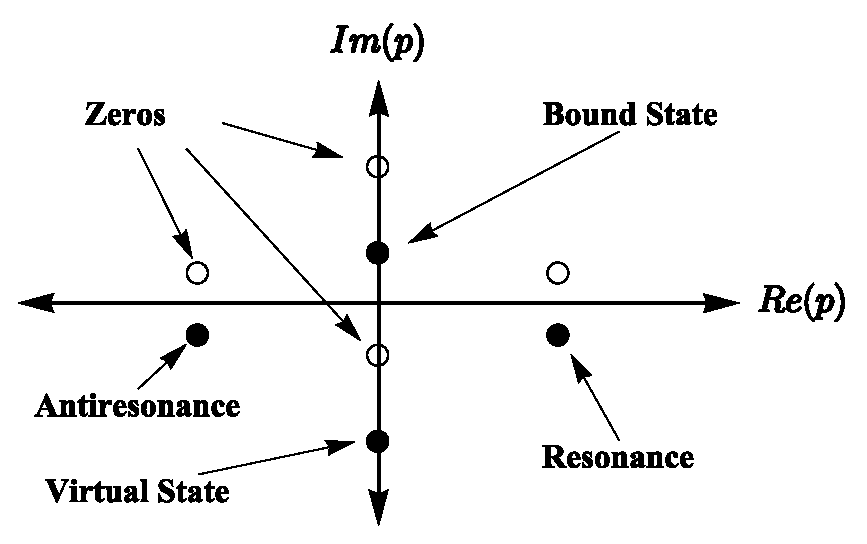
\includegraphics[width=0.75\linewidth]{Figures/DiagramPoles.eps}
	\caption{Example of configuration of  poles (filled circles) and zeros (empty circles) of the $S$-matrix eigenvalues in the complex momentum plane for hermitian Hamiltonians.  Poles in the upper half plane ($\operatorname{Im}(p) > 0$) correspond to bound eigenstates of the Hamiltonian, i.e. localized states with negative energy. Poles in the lower half plane correspond to  virtual states ($\operatorname{Re}(p) = 0$), resonances ($\operatorname{Re}(p) > 0$) and antiresonances ($\operatorname{Re}(p)<0$). The singularities with negative imaginary part correspond to states that do not belong to the Hilbert space since they are not normalizable. However, they can produce observable effects in the scattering amplitudes, in particular when they approach the real axis. The pole structure of symmetries IV, V, and VII, see Table \ref{tab:chapter2_Symmetries},
	is similar, but pole pairs are also possible in the upper half-plane.}
	\label{fig:DiagramPoles}
\end{figure}

%however generally do not conserve norm, and typically have complex eigenvalues and asymmetrical singularities of $S$.
%Surprisingly, as . After the proposal to realize PT-symmetric Hamiltonians
%in optical waveguides with gain and loss \cite{ruschhaupt2005physical}, the experimental realization of PT-symmetric structures has found many applications and triggered renewed interest in NH interactions.

% \comment{[Unknown citation here, What is Wang?]}.%\cite{Nixon2016,Chen2017,Yang2017,Wang}

%The reality of eigenvalues and finite matrices has been investigated in \cite{Bender2010}.
%However, arguments valid for finite matrices are not necessarily applicable
%to scattering systems with a continuum spectrum. In scattering systems it is also of interest to determine the general structure of $S$-matrix singularities in the complex momentum plane, including not only eigenvalues of $H$
%in the upper half-plane but also poles in the lower half plane such as resonances, antiresonances, and anti-bound states.
%Moreover, studies on systems with a continuum, often rely on
%local potentials, but non-local potentials are physically meaningful, they follow from Feschbach's projection,
%and offer richer possibilities.


%In this paper we study the symmetry properties of the $S$-matrix in the complex momentum plane for non-hermitian,
%non-local scattering Hamiltonians in one dimension.
%\blue{Specifically the goal of the paper is to show that a family of Hamiltonian symmetries characterized by antiunitary superoperators
%necessarily imply that the $S$-matrix singularities are either real or appear in conjugate pairs \textbf{(This was already noticed by Mostafazadehfazadeh. A new and more ambitious goal would be proving that if the Hamiltonian is invariant under the action of some antilinear superoperator, not necessarily unitary, the eigenenergies are real or come in complex conjugate pairs)}}. This structure implies the stability of bound and antibound states:   under these conditions a single discrete real singularity cannot bifurcate into a complex conjugate pair when deforming the potential.
%A complex pair can only appear when two real eigenvalues collide.

%\red{paper structure here}

The remainder of the article is organized as follows. In section \ref{sec:SymTheory} we review the scattering properties of eight different Hamiltonian symmetries. These symmetries may be characterized as commutativity or pseudohermiticity with respect to four unitary or antiunitary operators forming a Klein $4$-group, or as invariance with respect to the action of eight linear or antilinear superoperators. In section \ref{sec:chapter2_SPoles} we discuss the physical consequences of the symmetries in the pole structure of the scattering matrix eigenvalues  and hence in the transmission/reflection amplitudes. Four symmetries are shown to lead to complex poles corresponding to real energies or conjugate (energy) pairs.  In section \ref{sec:chapter2_separablePotentials} we exemplify the general results with separable potentials exhibiting parity-pseudohermiticity and time-reversal symmetry. These are the two non-trivial symmetries of the four (in the sense that the other two, hermiticity and PT-symmetry, are already well discussed). In section \ref{sec:RealEigenConclusions} we discuss and summarize our results.

\begin{landscape}
	\begin{table}
		\centering
		\caption{Symmetries of the potential based on the commutativity or pseudohermiticity of $H$ with the elements of $\mathbf{K}_4$ (column 2). Columns 3, 5, and 7 to 11 are to be read as follows: For each symmetry the object in the column is equal to the one in the top row of the column. The relations among potential matrix elements are given in coordinate and momentum representations in the third and fifth columns. In columns 4 and 6, each symmetry is regarded as the invariance of the potential with respect to the transformations represented by superoperators ${\cal L}$ (see Sec. \ref{sec:chapter2_super}) in coordinate  or momentum  representation.
		The fifth column gives the relations they imply in the matrix elements of $S$ and $\widehat{S}$ matrices. The final four columns set the relations for the scattering amplitudes.
		\vspace*{.2cm}
		\label{tab:chapter2_Symmetries}}
		\scalebox{1}{
		\begin{tabular}{ccccccccccc}
			%\hline
			1&2&3&4&5&6&7&8&9&10&11
			\\
			Code & Symmetry&  $\la x|V|y\ra$ & ${\cal{L}}$(coord)& $\la p|V|p'\ra$ & ${\cal L}$(momentum) &$\la p|S|p'\ra$ & $T^l$ & $T^r$ & $R^l$& $R^r$
			\\
			\hline
			I & $1H=H1$ &   $\la x|V|y\ra$ & ${ 1}$ &$\la p|V|p'\ra$ &${ 1}$& $\la p|S|p'\ra$ & $T^l$ & $T^r$ & $R^l$ & $R^r$
			\\
			II & $1H=H^\dagger 1$ &  $\la y|V|x\ra^*$ & ${\cal TC}$& $\la p'|V|p\ra^*$ &${\cal T'C'}$&$\la p|\widehat{S}|p'\ra$ & $\widehat{T}^l$& $\widehat{T}^r$ & $\widehat{R}^l$ & $\widehat{R}^r$
			\\
			III & $\Pi H=H\Pi$ &  $\la -x|V|-y\ra$ &${\cal I}$&  $\la -p|V|-p'\ra$ &${\cal I'}$&$\la -p|S|-p'\ra$ & $T^r$ & $T^l$ & $R^r$ & $R^l$
			\\
			IV & $\Pi H=H^\dagger \Pi$ &  $\la -y|V|-x\ra^*$ &${\cal CTI}$& $\la -p'|V|-p\ra^*$ &${\cal C'T'I'}$& $\la -p|\widehat{S}|-p'\ra$ & $\widehat{T}^r$ & $\widehat{T}^l$ & $\widehat{R}^r$ & $\widehat{R}^l$
			\\
			V & $\Theta H=H\Theta$ &  $\la x|V|y\ra^*$&${\cal C}$& $\la -p|V|-p'\ra^*$ &${\cal I'C'}$& $\la -p'|\widehat{S}|-p\ra$ & $\widehat{T}^r$ & $\widehat{T}^l$ & $\widehat{R}^l$& $\widehat{R}^r$
			\\
			VI & $\Theta H=H^\dagger\Theta$ &  $\la y|V|x\ra$&${\cal T}$& $\la -p'|V|-p\ra$ &${\cal I'T'}$& $\la -p'|S|-p\ra$ & $T^r$& $T^l$ & $R^l$& $R^r$
			\\
			VII & $\Theta\Pi H=H\Theta \Pi$ &  $\la -x|V|-y\ra^*$ &${\cal IC}$& $\la p|V|p'\ra^*$ &${\cal C'}$& $\la p'|\widehat{S}|p\ra$ &$\widehat{T}^l$& $\widehat{T}^r$ & $\widehat{R}^r$& $\widehat{R}^l$
			\\
			VIII& $\Theta\Pi H=H^\dagger \Theta \Pi$ &  $\la -y|V|-x\ra$ &${\cal IT}$& $\la p'|V|p\ra$ &${\cal T'}$& $\la p'|S|p\ra$ & $T^l$ & $T^r$ & $R^r$ & $R^l$
			%\\
			%\hline
		\end{tabular}
		}
	\end{table}
\end{landscape}
% -------------------------------------------------------------------------------------------------

\section{Hamiltonian Symmetries}
\label{sec:SymTheory}
%
\subsection{Basic concepts and terminology}
%
Let us first clarify the terminology. Scattering Hamiltonians are the ones that can be written as the sum of kinetic energy $H_0 = {p^2}/({2m})$ operator and a potential energy operator $V$,
%
\begin{equation}
	H = H_0 + V.
	\label{eq:ScatteringHamiltonian}
\end{equation}
%
$V$ is in general non-local, i.e., it does not have the local form $\la x|V|x'\ra=\delta(x-x')V(x)$.
%Non-local potentials may be as physical as non-hermitian ones, and appear generically in Feshbach formalism as effective interactions \cite{feshbachPQ1,feshbachPQ2}. Non-local potentials also arise in the analysis of molecular orbits when using the Hartree-Fock theory \red{old stuff, difficult to find good refs.}.
Apart from their generic appearance in Feschbach's partitioning technique, see e.g. \cite{Ruschhaupt2004a},
non-local potentials   are quite common in models that discretize the coordinates at specific sites, as in tight-binding models.
These are widely used for describing condensed matter and ultracold atoms in a lattice. For example, the well known Bose-Hubbard model has been generalized to a non-Hermitian Hamiltonian to account for dissipation effects, see e.g. \cite{Hiller2006,Zhong2011}. However, here we limit ourselves to continuous-coordinate scattering models.\footnote{
Also, discrete Hamiltonian matrix models abound in many fields, for example quantum optics, in which rather than couplings
among different ``sites'' there are couplings among states or levels.
Thus a generalized concept of ``non-locality'' may be applied,
as being equivalent to non-zero non-diagonal elements in the chosen basis. The non-Hermitian symmetry groups in these discrete models
can be larger than the set of symmetries based on eqs. (\ref{gs1}) and (\ref{gs2}) described here, which are constrained by the structure of $H_0$. Discrete model symmetries, interesting as they are, and
with potential applications in condensed matter, optics, or quantum optics,
lie beyond the scope of this work and need a deeper separate study.}
The potential function in position coordinates $V(x,x') = \bra{x}V\ket{x'}$ is assumed to decay fast enough to 0 when a position goes to infinity so that the usual operators of scattering theory are well defined and the Hilbert space is (biorthogonally) decomposed into a continuum
part with real eigenvalues and a discrete part. See Appendix \ref{Appendix:ScattFormalism} for a review of the formalism and notation we use.

We will now discuss the eight symmetries identified in \cite{Ruschhaupt2017},
which are associated with the two generalized symmetry relations corresponding to commutation with $A$ and $A$-pseudohermiticity \cite{Mostafazadeh2002}, see eqs. (\ref{gs1},\ref{gs2}).
%
%\begin{eqnarray}
%AH&=&HA,
%\label{gs1}
%\\
%AH&=&H^\dagger A,
%\label{gs2}
%\end{equation}a
%
%where $A$ is a unitary or antiunitary operator in Klein $4$-group $\mathbf{K}_4 = \left\{1,\Pi,\Theta,\Theta\Pi\right\}$ formed by the identity ($1$), parity ($\Pi$), time-reversal ($\Theta$) and their product ($\Theta\Pi$), also known as the PT operator.
We use Roman numeral to label these symmetries as shown in Table \ref{tab:chapter2_Symmetries}: I ($1H=H1$, the trivial identity)
; II ($1H=H^\dagger 1$, hermiticity or ``1-pseudohermiticity''); III ($\Pi H=H\Pi$, parity); IV ($\Pi H=H^\dagger \Pi$, $\Pi$-pseudohermiticity);  V ($\Theta H=H\Theta$, time-reversal invariance);  VI ($\Theta H=H^\dagger \Theta$, $\Theta$-pseudohermiticity);
VII ($\Pi\Theta H=H\Pi\Theta$, PT-symmetry); VIII ($\Pi\Theta H=H\Pi\Theta$, $\Pi\Theta$-pseudohermiticity).
Note that a local potential would automatically fulfill symmetry VI but this symmetry does not necessarily imply locality.
For local potentials four of the eight symmetries coincide with the other four \cite{Ruschhaupt2017}. Here we consider general nonlocal potentials where all the eight symmetries are distinct.


The generalization of the symmetry concept to the pair \eqref{gs1} and \eqref{gs2} is in fact quite natural if we take into account that a NH-$H$
has generically different left and right eigenvectors. Given a right eigenstate $\ket{\psi}$ of $H$ with eigenvalue $E$, Eq. (\ref{gs1}) implies that  $A|\psi\ra$ is also a right eigenvector with eigenvalue $E$ or $E^*$, whereas Eq. (\ref{gs2}) implies that $\la \psi|A$ is a left eigenvector of $H$ with eigenvalues $E^*$ or $E$,  for $A$ unitary or antiunitary respectively. \footnote{$A$ is an antiunitary operator if it is an antilinear operator that maps a Hilbert space onto itself satisfying $\expval{A \psi,A\phi}= \expval{\phi,\psi}$ for $\psi$ and $\phi$ in that Hilbert space. It  satisfies $AA^{\dagger}=A^\dagger A=1$, where the adjoint is to be understood as for antilinear operators, namely  $\expval{\phi,A^\dagger\psi} = \expval{\psi,A \phi}$ \cite{Muga2004}.}

The symmetries which imply the presence of real or complex-conjugate pairs of energy eigenvalues for bound eigenstates
are II, IV,V and VII.
The emergence of these complex-conjugate pairs has been previously discussed in \cite{Mostafazadeh2002,Bender2010} for a general class of diagonalizable Hamiltonians that posses a discrete spectrum. They can be heuristically understood for the symmetries we consider as follows: Symmetry V implies that the Hamiltonian must be real in coordinate space, which would lead to a real characteristic polynomial with real or complex-conjugate roots. Symmetry VII is PT symmetry which is well discussed in the literature as having real or complex-conjugate pairs of eigenvalues \cite{Bender1998}. Note also that the matrix elements of PT-symmetric Hamiltonians are real in the momentum representation. More generally, in \cite{Mostafazadeh2002b}, it was shown, for diagonalizable Hamiltonians having a discrete spectrum, that $A$-pseudohermiticity for a Hermitian invertible linear operator $A$ is equivalent to the presence of an ordinary symmetry of the form $BH = HB$ for some antilinear operator $B$ with $B^2 = 1$. Because $B$ is an antilinear operator, the eigenvectors $\ket{E_n}$  of $H$ with eigenvalues $E_n$ satisfy
%
\begin{eqnarray}
	H B \ket{E_n}&=&B H \ket{E_n} \nonumber \\
	&=&E_{n}^{*} B \ket{E_n}.
\end{eqnarray}
%
Therefore complex eigenvalues $E_n$ come in complex-conjugate pairs. In particular, when $\ket{E_n}$  is an eigenvector of $B$, i.e., $B\ket{E_n} = e^{ib_n} \ket{E_n}$ for some real number $b_n$, we have $E_n \in \mathbb{R}$.
The proof of the equivalence of $A$-pseudohermiticity for linear $A$ and the presence of ordinary antilinear symmetries given in \cite{Mostafazadeh2002b} relies on the observation that every diagonalizable Hamiltonian with a discrete spectrum is $\tau$-pseudohermitian for some invertible Hermitian antilinear operator $\tau$, i.e.,
$\tau H = H^\dagger\tau$. This relation together with Eq. (\ref{gs2}) implies $BH = HB$,
if we set $B = A^{-1}\tau$. (If $AH=H^\dagger A$ and $A$ is a Hermitian antilinear operator, a linear $B = A^{-1}\tau$ can also be constructed so that $BH=HB$, but the $E_n$ do not form conjugate pairs.)
In Appendix \ref{Appendix:AlternativeFormulationOfPseudoHermiticity} we extend this construction to scattering potentials.

In summary, the symmetries with conjugate pairs II, IV, V, and VII can be all expressed as the commutation of $H$ with a certain antilinear operator, as seen directly in the symmetries V and VII, in which $H$ commutes with an antilinear $A$,  and by constructing an antilinear $B$ in the symmetries II and IV.
A novel aspect uncovered in this paper is that whenever one of  the above-mentioned four symmetries holds not only the complex eigenvalues representing the bound states come in conjugate-complex pairs, but all the complex poles of the $S$-matrix have this property.

%
%
\subsection{Superoperator formalism \label{sec:chapter2_super}}
The eight symmetries listed in Table \ref{tab:chapter2_Symmetries} may also be regarded as the invariance
of the Hamiltonian matrix with respect to
transformations represented by superoperators ${\cal L}$ \cite{Simon2018} defined by
%
\begin{eqnarray}
	\mathcal{L}(H)=
	\begin{cases}
		A^\dagger H A &  \text{I, III,V,VII} \\
		A^\dagger H^\dagger A &\text{II, IV, VI, VIII}
		\end{cases}.
\end{eqnarray}
%
%\red{Write how the symmetries look like using the superoperator formalism in position and mommentum basis.}
%
%
%We adhere to the simple definition of symmetry as stated by Feynman, which he attributed to Weyl:
%``a thing is symmetrical if one can subject it to a certain operation and it appears exactly the same after the operation'' \red{citation}.
This definition of the superoperator action is independent of the representation we use, but its realization
in coordinates or momenta in terms of the operations of complex conjugation, transposition, and inversion is different.
For example, in coordinate representation, these superoperators take the following forms (see column 3 in Table \ref{tab:chapter2_Symmetries}),
%
\begin{eqnarray}
	1 H&=&\int\!\!\int |x\ra \la x|H|y\ra\la y| dx dy,
	\nonumber\\
	{\cal T} (H) &=&\int\!\!\int |x\ra \la y|H|x\ra\la y| dx dy,
	\nonumber\\
	{\cal C} (H)&=&\int\!\!\int |x\ra \la x|H|y\ra^*\la y| dx dy,
	\nonumber\\
	{\cal I} (H)&=&\int\!\!\int |x\ra \la -x|H|-y\ra\la y| dx dy.
	%\nonumber\\
	%{\cal CT} H &=&\int\!\!\int |x\ra \la y|H|x\ra^*\la y| dx dy,
	%\nonumber\\
	%{\cal CI} H&=&\int\!\!\int |x\ra \la -x|H|-y\ra^*\la y| dx dy,
	%\nonumber\\
	%{\cal TI} H&=&\int\!\!\int |x\ra \la -y|H|-x\ra\la y| dx dy,
	%\nonumber\\
	%{\cal CTI} H&=&\int\!\!\int |x\ra \la -y|H|-x\ra^*\la y| dx dy,
	\label{defs}
\end{eqnarray}
%
% inner product for linear operators F and G, hhF|Gii = trF�G, we can show that all the above superoperators L are either unitary (for L = 1, T , I, T T ) or antiunitary ( for {\cal L} = C, CT , CI, CT I). Recall the following definition of unitarity and antiunitarity.
Adopting the following inner product for linear operators $F$ and $G$,\linebreak $\langle\langle F|G\rangle\rangle={\rm{tr}} F^\dagger G$,
we can show that all superoperators ${\cal L}$ are either unitary (for ${\cal L}=1,{\cal T},{\cal I},{\cal TI}$), or antiunitary (for ${\cal L}={\cal C}, {\cal CT},{\cal CI},{\cal CTI}$), as defined by
%
\begin{eqnarray}
	\langle\langle {\cal L}F| {\cal L}G\rangle\rangle&=& \langle\langle F| G\rangle\rangle\;\;\;  ({\cal L}\; {\rm unitary}),
	\\
	\langle\langle {\cal L}F| {\cal L} G\rangle\rangle&=& \langle\langle  F| G\rangle\rangle^*\;\;\;  ({\cal L}\; {\rm antiunitary}).
\end{eqnarray}
%
They all satisfy ${\cal L}{\cal L}^\dagger={\cal L}^\dagger {\cal L}=1$
where the adjoints are defined differently for linear or antilinear superoperators,
\begin{eqnarray}
	\langle\langle F| {\cal L}^\dagger G\rangle\rangle&=& \langle\langle {\cal L} F| G\rangle\rangle\;\;\;  ({\cal L}\; {\rm unitary}),
	\\
	\langle\langle F| {\cal L}^\dagger G\rangle\rangle&=& \langle\langle {\cal L} F| G\rangle\rangle^*\;  ({\cal L}\; {\rm antiunitary}).
\end{eqnarray}
%
Moreover the eight superoperators  satisfy ${\cal L}^\dagger={\cal L}$.

The set $\{1, \cal{I,T,C,CT,TI,IC,CTI}\}$ forms the elementary abelian group $E8$ \cite{Rose2009}.
%and cite. Ref: Rose, H. E. A course on finite groups. Springer-Verlag: London, UK, 2009, ISBN 978-1-84882-888-9.}.
This is a homocyclic group, namely, the direct product of isomorphic
cyclic groups of order 2 with generators $\cal{C,T,I}$. We may, similarly to Eq. (\ref{defs}), define primmed superoperators in momentum representation, e.g. \linebreak ${\cal T'} H =\int\!\!\int |p\ra \la p'|H|p\ra\la p'| dp dp'$. They also form the E8 group \linebreak $\{1, \cal{I',T',C',C'T',T'I',I'C',C'T'I'}\}$. Only for the subgroup $\{1, \cal{I,CT,CTI}\}$ the superoperators have the same representation-independent form in terms of complex conjugation, transposition and inversion.

A direct application of the superoperator framework is the generalization of Wigner's
formulation of symmetries \cite{Wigner1959}. He associated symmetry transformations to unitary or antiunitary operators preserving the (Hilbert space) inner product, namely the ``transition probabilities'' $|\expval{A\psi,A\phi}|^2=|\expval{\psi,\phi}|^2$.
For general states described by density operators $\rho_1,\rho_2$, transition probabilities are computed as $\la\la \rho_1|\rho_2\ra\ra$
and the transformations described by the unitary or antiunitary superoperators preserve the
transition probability. Hamiltonian symmetries are, within the conventional Wigner scheme, the  symmetry transformations that leave the Hamiltonian invariant ($A^\dagger H A=H$, so that $A$ and $H$ commute). Here the Hamiltonian symmetry is more broadly defined  as
the invariance ${\cal L}H=H$, which includes transformations  beyond the conventional scheme.


%
%
%

%A further alternative view of the eight symmetries generalizes results found for discrete Hamiltonians that show that
%symmetries of the form (\ref{gs2}) may in fact be also formulated as commutation relations between $H$ and certain operators, linear
%for antilinear $A$, and antilinear for linear $A$. The generalization for scattering Hamiltonians and the explicit construction
%of the operator that commutes with $H$ is worked out in the Appendices.
%
\section{S-matrix pole structure}
\label{sec:chapter2_SPoles}
%
%One of the most studied aspects of the collisions with non-hermitian potentials is the meaning
%of poles of $S_j(p)$ in the complex plane $p$ and their motions. In the unitary case
%the poles of the amplitudes $S_j(p)$ are classiffied according to their position in the plane: the poles
%on the positive imaginary axis correspond to bound states, those in the fourth quadrant to resonances,
%and in the third quadrant to antiresonances. The non-unitary case presents new possibilities:
%poles in the first  quadrant, corresponding to states whose norm grows exponentially with time, and
%poles in the second quadrant, corresponding to states whose norm decreases with time [31]. The poles
%in the upper half-plane are on the first  Riemann sheet of the energy so the corresponding energy
%belongs to the point spectrum of $H$. In the hermitian case ($S =\widehat{S}$) the poles in the lower momentum
%half-plane come in symmetrical pairs with respect to the imaginary axis, with zeroes in the upper
%half-plane at conjugate positions but this symmetrical pattern is broken
%in general for non-hermitian Hamiltonians. Exceptions to this will be presented in Section .... .
%
%
To derive the results in \cite{Ruschhaupt2017} an extensive use of the scattering matrix ($S$-matrix) formalism was made. The full $S$-matrix
provides outgoing waves when acting on incoming waves. It is typically decomposed into on-the-energy-shell matrices.
%is simply the operator that acting on an incoming wave function gives the resulting wave function after the scattering has taken place. The relations in \eqref{gs1} and \eqref{gs2} imply certain intertwining relations of the $S-$matrix with the elements of the Klein's group that lead to the selection rules in  \cite{Ruschhaupt2017}.}
In 1D scattering, the on-the-energy-shell $\sf{S}(p)$ matrix for $H$ is defined on the real positive momentum axis in terms of transmission and reflection amplitudes for right
and left incidence \cite{Muga2004},
%
\begin{equation}
	\sf{S}=\left(\begin{array}{cc}
	T^l(p)&R^r(p)
	\\
	R^l(p)&T^r(p)
	\end{array}\right).
\end{equation}
%
There is a companion matrix $\widehat{\sf{S}}$ with hatted amplitudes corresponding to scattering by $H^{\dagger}$. See Appendix \ref{Appendix:ScattFormalism} and \cite{Muga2004} for details. The $\sf{S}$ matrix contains the scattering amplitudes for incoming wave packets with well defined momentum being scattered into states with the same kinetic energy and reflected and transmitted components.
%
For negative $p$ the matrix elements give the amplitudes of scattering states with a pure outgoing plane wave towards the right or the left.
Moreover we assume, as it is customary,
that the amplitudes may be continued analytically beyond the real axis.
The existence of a continuation on a complex plane domain depends on decay properties of the potentials and may
be checked for each potential.
The analytical continuation is indeed possible for the model potentials of the following section.



The eigenvalues of $\sf{S}$ can be calculated from the transmission and reflection amplitudes as
%
\begin{equation}
	S_j=\frac{(T^l+T^r)+(-1)^j[(T^l-T^r)^2+4R^lR^r]^{1/2}}{2}
	\label{Sform}
\end{equation}
%
for $j=1,2$, and of course there is a similar expression for $\widehat{S}_j$ with hatted amplitudes.
In general they satisfy the relations \cite{Muga2004},
%
\begin{equation}\label{pam1}
	S_j(p)=\widehat{S}_j^*(-p^*)\,,
\end{equation}
%
and
%
\begin{equation}\label{pam2}
	\widehat{S}_j^*(p^*)S_j(p)=1\,.
\end{equation}
%
Combining eqs. (\ref{pam1}) and (\ref{pam2}) gives
%
\begin{equation}\label{pam3}
	S_j(p)=S^{-1}_j(-p)\,.
\end{equation}
%
Equation \eqref{pam3} is remarkable since it reveals the presence of a pole (zero) at $-p$ if there is a zero (pole) at $p$.
%
%Of
%Generalizing the concept of symmetry for NH-Hamiltonians, eight symmetries are identified, see Table \ref{tab:chapter2_Symmetries},
%among which four imply
%a structure for poles and zeros of the S matrix compatible with the existence of real, discrete eigenvalues, more specifically, the discrete eigenvalues
%appear necessarily in conjugate pairs. Two of these
%four symmetries are well known, namely, hermiticity and PT-symmetry, whereas the other two types are denominated here as parity pseudohermiticity (symmetry type IV)
%and time-reversal invariance (symmetry type V).
If the following relations are fulfilled,
%
\begin{eqnarray}
	T^{r,l}(p)&=&\widehat{T}^{r,l}(p)\; {\rm or}\; T^{r,l}(p)=\widehat{T}^{l,r}(p),
	\label{ts}
	\\
	R^{r,l}(p)&=&\widehat{R}^{r,l}(p)\; {\rm or}\; R^{r,l}(p)=\widehat{R}^{l,r}(p),
	\label{rs}
\end{eqnarray}
%
then
%
\begin{equation}
	S_j(p)=\widehat{S}_j(p),
\end{equation}
%
which together with Eq. \eqref{pam1} gives
%
\begin{equation}
	S_j(p)=S_j^*(-p^*).
	\label{eq:PoleSymmetry}
\end{equation}
%}
In plain language, Eq. \eqref{eq:PoleSymmetry} tells that if eqs. (\ref{ts}) and (\ref{rs}) are satisfied,  the poles and zeros of $S_j$ must be symmetrically distributed with respect to the imaginary axis of momentum complex plane. Combined with Eq. (\ref{pam3})
this also means that each pole has a symmetrical zero with respect to the real axis. This symmetrical distribution of poles and zeros is the same as in the Hermitian case (see fig. \ref{fig:DiagramPoles}),
%end red
the only difference being the possibility
of finding pairs of symmetrical poles in the upper complex plane when $H\neq H^\dagger$. They represent normalizable ``bound states
with complex energies''. When they  are not present, the discrete spectrum becomes purely real.

According to Table \ref{tab:chapter2_Symmetries},  eqs. (\ref{ts}) and (\ref{rs}) are fulfilled
for symmetries  II (hermiticity), VII (PT-symmetry), IV (parity pseudohermiticity),
and V (time-reversal invariance). Thus, Hamiltonians having these symmetries have their $S-$matrix poles symmetrically distributed around the imaginary axis. For local potentials the last two symmetries coalesce with the first two well-known
cases \cite{Ruschhaupt2017}, namely,
IV becomes equivalent to PT-symmetry, and V becomes equivalent to hermiticity. For non-local potentials, though, these symmetries
correspond to genuinely distinct properties. In the following section we shall demonstrate this fact with potentials that are
either purely parity-pseudohermitian (and not PT-symmetrical), or time-reversal invariant but not Hermitian.
%
\section{Separable Potentials}
\label{sec:chapter2_separablePotentials}
%
%
In order to illustrate and test the theoretical concepts that we have discussed, in particular the
symmetrical configuration of poles with respect to the imaginary axis in the complex momentum plane for certain Hamiltonian symmetries, we will use some solvable toy models consisting on rank-one separable potentials.
Separable potentials are quite useful models as a solvable approximation to realistic ones, in particular in nuclear, atomic and molecular physics \cite{Popov2019}.
Often they lead to explicit expressions
for wave functions or scattering amplitudes, so they are used to test concepts and new methods.
They are also instrumental in learning about different dynamical phenomena (for example transient effects, short-time and long-time behavior, or anomalous decay laws)  and their relation to complex-plane singularities
\cite{Muga1990,Muga1996,Muga1996a,Muga1998}. Their simplest version takes the form
$|\chi\ra V_0\la\chi|$ for some  $\chi$.   In particular, with a complex $V_0$,
they have been used to examine anomalous (negative) time delays caused by  crossing of zeroes of the $S$-matrix eigenvalues or $S$-matrix elements across the momentum real axis \cite{Muga1998a}.

In this work we consider the simple structure
$V=V_0 \ketbra{\phi}{\chi}$, with $V_0$ (potential strength) real, and conveniently chosen functions $\phi$, $\chi$.
The aim of this section is to demonstrate the formal results of the previous section without attempting to simulate any specific systems, but we note that separable, NH potentials are instrumental to model nuclear reactions, in particular  by increasing the rank (number of separable terms) \cite{Hlophe2017}.
Separable NH potentials also provide solvable approximations to nonlocal NH potentials that arise naturally in quantum optics to describe the interaction of a ground state atom with a laser beam \cite{Ruschhaupt2004a}.

In passing we shall also note some interesting phenomena that may be studied in more detail elsewhere, such as pole collisions, crossings of
the real axis, or diodic (Maxwell demon) behavior with asymmetrical transmission for right/left incidence.

From the stationary Schr\"{o}dinger equation $H \ket{\psi} = E \ket{\psi}$, the eigenvalues of separable potentials may be found by solving
%
\begin{eqnarray}
	Q_{0}(E)V_{0} = 1,
	\label{roots}
\end{eqnarray}
%
where $Q_{0}(E)=\bra{\chi}(E-H_0)^{-1}\ket{\phi}$ and $H_{0}=p^{2}/(2m)$. Moreover, for a separable potential, the transition operator $T_{op}$ can be written (see Appendix \ref{Appendix:SeparablePotentials_TransitionOperator}) as
%
\begin{equation}
	T_{op}=\frac{V_{0}}{1-V_{0} Q_{0}(E)} \ketbra{\phi}{\chi}.
\end{equation}
%
Since all scattering amplitudes in $S$ are simply related to matrix elements of $T_{op}$ in momentum representation, see
Eq. (\ref{art}), solutions to Eq. (\ref{roots}) provide their core singularities (independent of the representation \cite{Muga1996}).
%In the upper momentum plane they correspond to the discrete spectrum of $H$. In the lower half-plane they are
%resonances (fourth  quadrant), antiresonances (third quadrant), or virtual states (on the imaginary axis).
Once $Q_{0}(E)$  is calculated, the transmission and reflection amplitudes can be found from \eqref{art}
using the momentum representation of $\ket{\phi}$ and $\ket{\chi}$.

In the following subsections we will build a Hamiltonian with symmetry V (time reversal) and another one with symmetry IV
(parity pseudohermicity) and illustrate the symmetries of the $S$ matrix poles in momentum complex plane.

%
\subsection{Time-reversal symmetric potential}
%
%
\begin{figure}[h]
	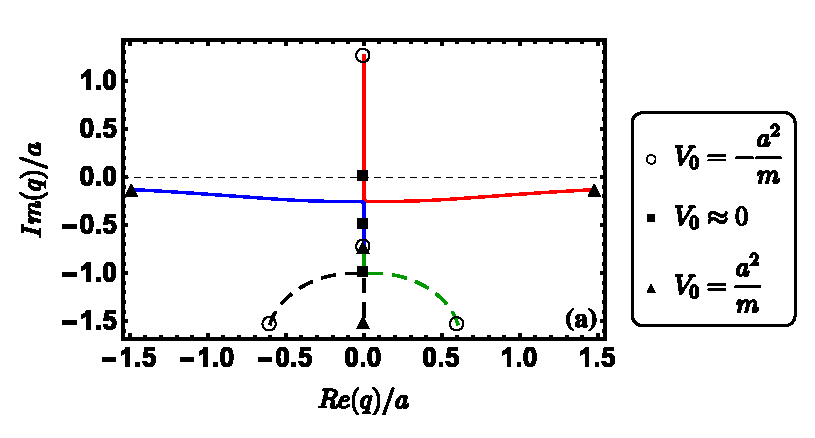
\includegraphics[width=1.0\linewidth]{Figures/VSymEigenvalsVaryingV0_Momentum.eps}
	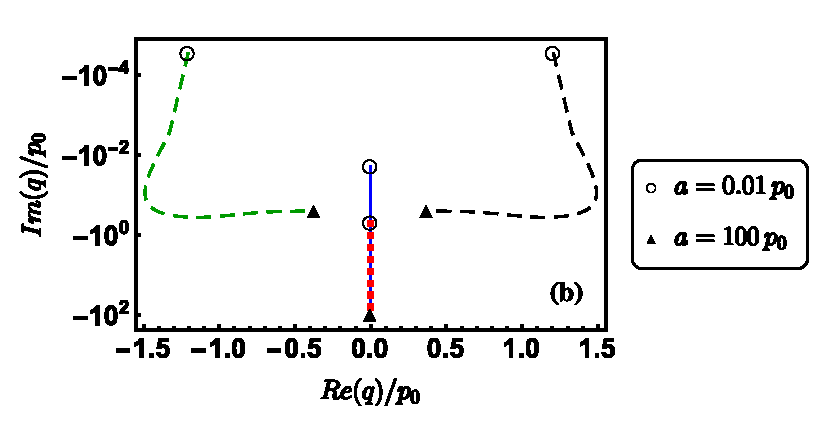
\includegraphics[width=1.0\linewidth]{Figures/VSymEigenvalsVaryingA_Momentum_Log.eps}
	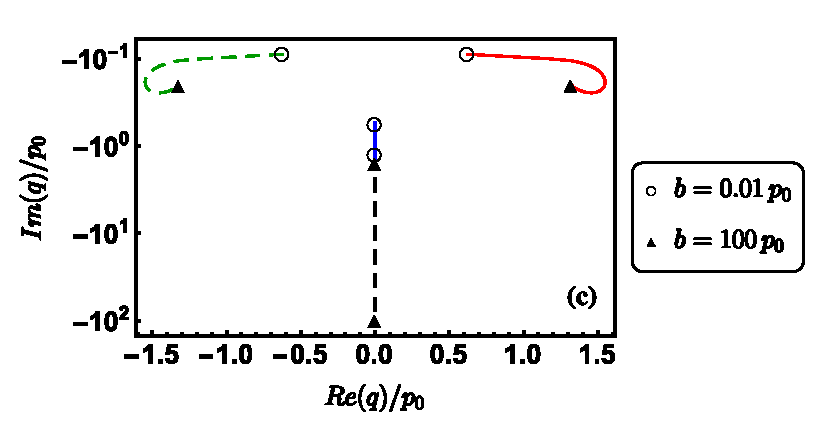
\includegraphics[width=1.0\linewidth]{Figures/VSymEigenvalsVaryingB_Momentum_Log.eps}
	\caption{(Color online) Poles and pole trajectories of time-reversal symmetric potential \eqref{TRpot} for (a) varying $V_0$ with $a=2 b$; (b) varying $a$ with $b=0.5\, p_0$, $V_0>0$; and (c) varying $b$ with $a=p_0$,
	$V_0>0$. At pole collisions we connect each of the incoming trajectories with a different emerging trajectory but the choice of outgoing branch  is arbitrary since the two colliding poles lose their identity.}
	\label{fig:VSymEigenvals}
\end{figure}

We start with an example of a separable potential which only satisfies symmetry V (apart from the trivial symmetry I). The normalised vector $\ket{\chi}$, is given in position and momentum representation as
%
\begin{eqnarray}
	\braket{x}{\chi}&=&\sqrt{\frac{a}{\hbar}} e^{-a \left| x \right|/\hbar},
	\nonumber \\
	\braket{p}{\chi}&=& \sqrt{\frac{2 a^3}{\pi}} \frac{1}{p^2+a^2}.
\end{eqnarray}
%
We choose $\ket{\phi}$ similarly as
%
\begin{eqnarray}
	\braket{x}{\phi}=&\sqrt{\frac{2ab}{\hbar (a+b)}} \begin{cases}
	e^{-b x/\hbar} &x>0,\\ e^{a x/\hbar}  &x<0,
	\end{cases}\nonumber \\
	\braket{p}{\phi}=& \sqrt{\frac{ab}{\pi (a+b)}}\frac{a+b}{(p+i a)(p-i b)}.
\end{eqnarray}
%
The real and positive parameters $\hbar/ a$ and $\hbar/ b$ determine the width of the potential functions in coordinate representation.
$b$ is chosen different from $a$ to introduce a right/left  asymmetry in $\braket{x}{\phi}$.
In coordinate representation the potential is given as
%
\begin{eqnarray}
	\la x|V|y\ra = V_{0} \sqrt{\frac{2 b a^2}{\hbar^2 (a+b)}} \begin{cases}
	e^{-(a \left| y \right|+b x)/\hbar} \, &x>0,\\ e^{a (x-\left| y \right|)/\hbar} \,  &x<0.
\end{cases} \label{TRpot}
\end{eqnarray}
%
%which can be seen in fig. \ref{fig:VSymPotentialPlot}.
Clearly the potential is always even in $y$ and in the limiting case where $a=b$, it is also even in $x$. For $a=b$, the potential will satisfy parity symmetry (III) and also PT symmetry (VII), without asymmetric transmission or reflection.
% so we ignore it hereafter.

We define first a complex momentum $q=\sqrt{2 m E}$ (for complex $E$) with positive imaginary part.
To calculate $Q_{0}(q)$ explicitly we use a closure relation in momentum representation, and
complex contour integration around the poles at $ia$, $q$ and $ib$.
The result is then analytically continued to the whole $q$-plane,
%
\begin{eqnarray}
&&Q_{0}(q)/m=
\nonumber\\
&&-\frac{i \sqrt{2b} \left[2 a (a+b)^2-q^2 (3 a+b)-i q (2 a+b) (3 a+b)\right]}{q (a+b)^{3/2} (a-i q)^2 (b-i q)},
\nonumber\\
\label{eq:ResolvantVSymm}
\end{eqnarray}
%
with which we may calculate the transmission and reflection amplitudes.
The four roots of Eq. (\ref{roots}) are the core poles.

Using $m$, $V_0$ and $\hbar$ we define the length and momentum scales $L_0 = \hbar/\sqrt{mV_0}$ and $p_0 = \sqrt{mV_0}$. In fig. \ref{fig:VSymEigenvals}(a), we can see the trajectory of the $S$-matrix core poles (zeros
of $1-V_0Q_0(q))$ for varying $V_0$. Notice a bound state for $V_0<0$ and collisions of the eigenvalue pairs around $V_0 = 0$. In figs. \ref{fig:VSymEigenvals}(b) and \ref{fig:VSymEigenvals}(c), where $V_0$ is positive and $a$ or $b$ are varied,
there are two virtual states and one resonance/anti-resonance pair. In all cases the symmetry of the poles about the imaginary axis
% for fig. \ref{fig:VSymEigenvals},
which corresponds to real energies or complex-conjugate pairs of energies, is evident. For larger values of the $a$ or $b$ parameters
(not shown)
the pair collides so that all poles end up as virtual states.

Figure \ref{fig:VSymScattAmplitudes} depicts the associated transmission and reflection coefficients (square moduli of the amplitudes) as functions of the momentum $p$. $|R^l(p)|=|R^r(p)|$ for all $p$ due to symmetry V \cite{Ruschhaupt2017}.
The coefficients can be greater than one in contrast to the Hermitian case.

%%%%%%%%%%%%%%%%%%%%%%%%%%%%%%%%%%%%%%%%%%
%Figure
%%%%%%%%%%%%%%%%%%%%%%%%%%%%%%%%%%%%%%%%%%
\begin{figure}
\begin{center}
	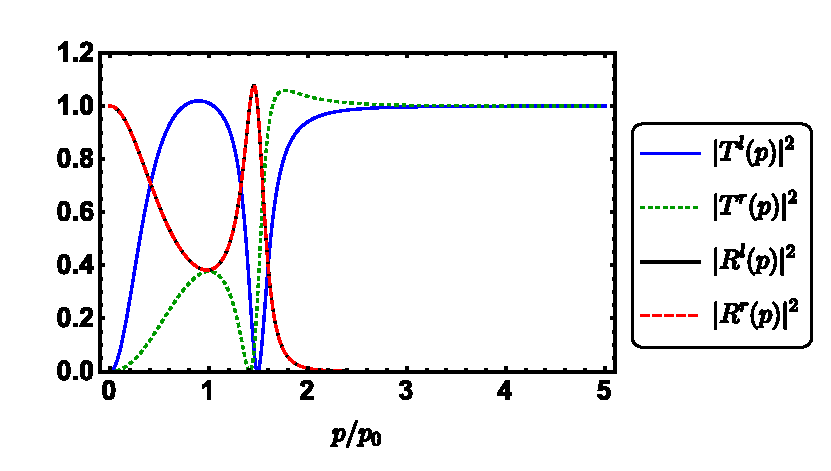
\includegraphics[width=1\linewidth]{Figures/VSymScattAmplitudes.eps}
\end{center}
\caption{(Color online) Transmission and reflection coefficients of the time-reversal symmetric potential \eqref{TRpot} with $a=p_0$, $b= 0.5\, p_0$ and $V_0>0$.}
\label{fig:VSymScattAmplitudes}
\end{figure}
%%%%%%%%%%%%%%%%%%%%%%%%%%%%%%%%%%%%%%%%%%

%
\subsection{Parity pseudohermitian potential}
%
%
As a second example we will consider  a separable potential which only fulfils symmetry IV. The normalised vector $\ket{\chi}$ in position and momentum representation is
%
\begin{eqnarray}
\braket{x}{\chi}=& \sqrt{\frac{a}{\hbar}} \begin{cases}
e^{-(a+ib)x/\hbar}  &x>0,\\ e^{a x/\hbar} &x<0,
\end{cases} \nonumber \\
\braket{p}{\chi}=&  \sqrt{\frac{a}{2\pi}} \frac{2 a+ i b}{(p+ia)(p+b-i a)},
\end{eqnarray}
%
where $a>0$ and $b$ is real.
We choose $\ket{\phi}$ as
%
\begin{eqnarray}
\braket{x}{\phi}=& \sqrt{\frac{a}{\hbar}} \begin{cases}
e^{-a x/\hbar} &x>0,\\ e^{(a+i b)x/\hbar} &x<0,
\end{cases} \nonumber \\
\braket{p}{\phi}=& \sqrt{\frac{a}{2\pi}} \frac{2 a+i b}{(p-ia)(p-b+i a)},
\end{eqnarray}
%
where $\hbar/a$ gives as before the width in coordinate representation. The potential functions in coordinate representation become asymmetrical
because of the  imaginary terms  $ib$ in  the exponent added only on  one side. This term leads to oscillations in real and imaginary parts. In momentum representation $b$ appears as a real shift in the position of one of the poles.
%
In coordinate representation the potential is
%
\begin{eqnarray}
\hspace*{-0.6cm}\la x|V|y\ra=  \frac{aV_{0}}{\hbar} \begin{cases}
e^{-\left[a (x+y) - i b y\right]/\hbar} \, ,&x>0,\,y>0\\
e^{a(y-x)/\hbar} \,  ,&x>0, \,y<0\\
e^{\left[a(x-y)+i b(x+y)\right]/\hbar} \,  ,&x<0,\,y>0\\
e^{\left[a(x+y)+i b x\right]/\hbar} \,  ,&x<0,\,y<0
\end{cases}.
\label{Ppot}
\end{eqnarray}
%
%see fig. \ref{fig:IVSymPotentialPlot}.
The case $b=0$ implies that the potential is real and hence satisfies time-reversal symmetry (V) with equal reflection amplitudes (as in the previous case), and also symmetry VIII.


\begin{figure}[h]
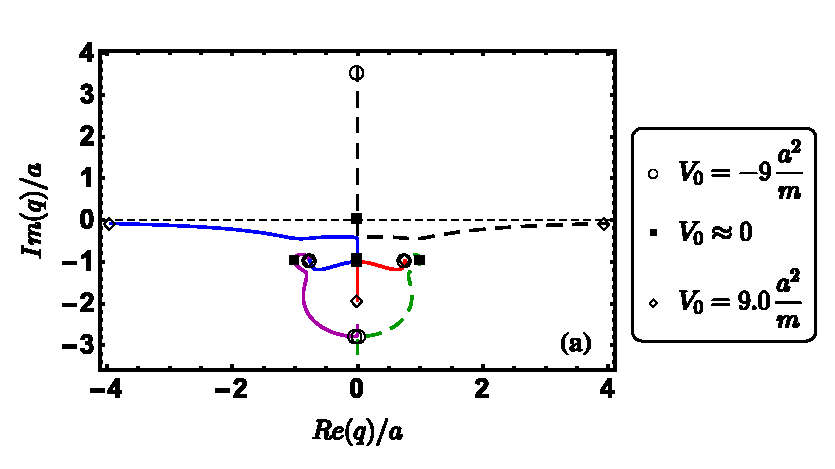
\includegraphics[width=1.0\linewidth]{Figures/IVSymEigenvalsVaryingV0new.eps}
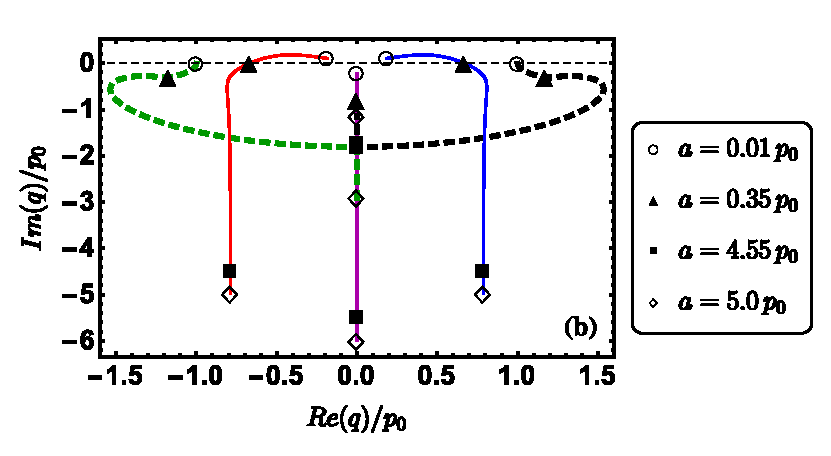
\includegraphics[width=1.0\linewidth]{Figures/IVSymEigenvalsVaryinganew.eps}
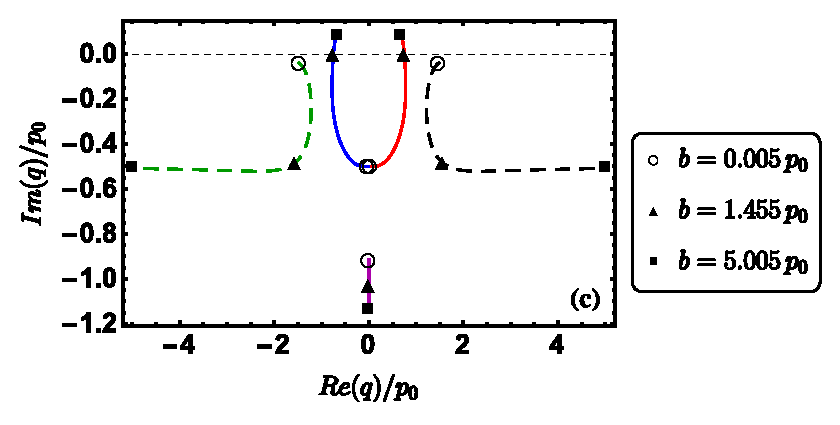
\includegraphics[width=1.0\linewidth]{Figures/IVSymEigenvalsVaryingbnew.eps}
\caption{(Color online) Poles and pole trajectories for the parity pseudohermitian potential \eqref{Ppot} (a) varying $V_0$ with $a=b$; (b) varying $a$ with $b=p_0$, $V_0>0$; (c) varying $b$ with $a=0.5\, p_0$, $V_0>0$.}
\label{fig:IVSymEigenvals}
\end{figure}



By calculating $Q_{0}$ again explicitly using complex contour integration around the poles at $-q$, $-b-i a$ and $b-i a$, we get that
%
\begin{eqnarray}
&&Q_{0}(q)/m
\nonumber\\
&&=\frac{8 a^2 q^3-4 a^2 q \left(10 a^2+b^2\right)-i a \left(4 a^2+b^2\right)^2+32 i a^3 q^2}{q \left(4 a^2+b^2\right) (a-i q)^2 \left[b^2+(a-i q)^2\right]}.
\nonumber\\
\end{eqnarray}
%
Equation \eqref{roots} has five roots in this case constituting core poles of the $S$ matrix elements.

Figure \ref{fig:IVSymEigenvals} depicts the trajectories of these poles for varying $a$, $b$ or $V_0$. As for the previous potential, the poles are symmetric with respect to the imaginary axis. In fig. \ref{fig:IVSymEigenvals}(a) there is a single bound state for $V_0<0$ while for positive values there are a resonance/antiresonance pair and a pair of virtual states. There are collisions of eigenvalues for values of $V_0$ close to 0. In fig. \ref{fig:IVSymEigenvals}(b)  two complex-conjugate (bound) eigenvalues cross the real axis and become a resonance/antiresonance pair. At the exact point where the eigenvalues are on the real axis, the scattering amplitudes diverge, however the eigenvalues of the $S$ matrix do not, since divergences of the left and right amplitudes cancel each other. For $a  \approx 4.55$ $p_0$ a resonance/antiresonance pair collides and becomes a pair of virtual states. In fig. \ref{fig:IVSymEigenvals}(c) another crossing of the real axis takes place, but in this case when decreasing $b$.

Figure \ref{fig:T_R_fig2} depicts the associated transmission and reflection coefficients as functions of the momentum $p$. The eigenvalues are not always equal since parity pseudohermicity does not imply any strict restriction to them \cite{Ruschhaupt2017}. For large  momenta, i.e. $p \gg \sqrt{2} p_0$, the potential is transparent giving $T^l,T^r \approx 1$. For $p\approx 1.5$ $p_0$ the right incidence transmission has a pronounced peak. Comparing with \ref{fig:IVSymEigenvals}(c), we notice that the values of the potential parameters and the momentum are close to the ones for which the real axis crossing takes place. Around $p = 0.6$ $p_0$ the potential acts as an asymmetric transmitter
%(\red{Use the same code as in the previous paper?:$\mathcal{TR/T,T/A,...}$}) device
\cite{Ruschhaupt2017}.


%%%%%%%%%%%%%%%%%%%%%%%%%%%%%%%%%%%%%%%%%%
%Figure
%%%%%%%%%%%%%%%%%%%%%%%%%%%%%%%%%%%%%%%%%%
\begin{figure}[t]
\begin{center}
	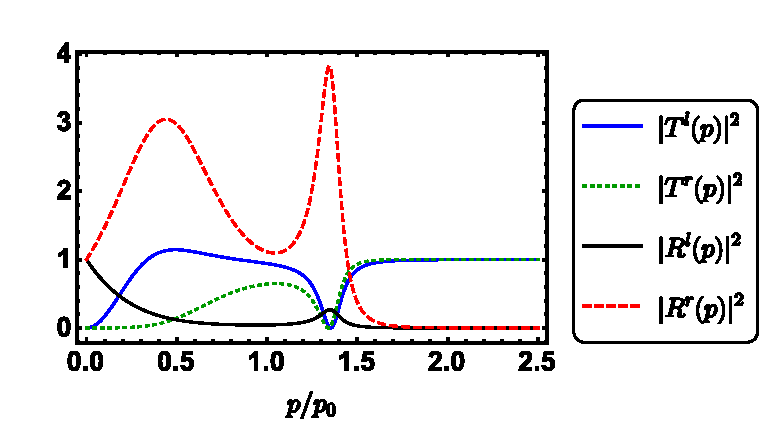
\includegraphics[width=\linewidth]{Figures/IVSymTR.eps}
\end{center}
\caption{(Color online) Transmission and reflection coefficients for $a=b=0.5\, p_0$ and $V_0>0$.}
\label{fig:T_R_fig2}
\end{figure}
%%%%%%%%%%%%%%%%%%%%%%%%%%%%%%%%%%%%%%%%%%

%%%%%%%%%%%%%%%%%%%%%%%%%%%%%%%%%%%%%%%%%%
%Figure
%%%%%%%%%%%%%%%%%%%%%%%%%%%%%%%%%%%%%%%%%%

%%%%%%%%%%%%%%%%%%%%%%%%%%%%%%%%%%%%%%%%%%

%\subsection{Symmetry VI example?}
%
%\red{Include other results here}

\section{Conclusion}
\label{sec:RealEigenConclusions}

In this paper we have studied some aspects of the scattering of a structureless particle in one dimension by
generally non-local and non-Hermitian potentials.
%Regarding
%the location of poles of the $S$ matrix eigenvalues in the momentum complex plane,
Conditions that were found for discrete Hamiltonians to imply conjugate pairs of discrete eigenenergies
(pseudohermiticity with respect to a linear operator or commutativity of $H$ with an antilinear operator \cite{Mostafazadeh2002,Mostafazadeh2002a,Mostafazadeh2002b}) can in fact be extended to scattering Hamiltonians in the continuum, implying symmetry relations not just for bound-state eigenvalues
but also for complex
poles of the $S$-matrix. Specifically the poles of $S$ matrix eigenvalues
are symmetrically located with respect to the imaginary axis, also in the lower momentum plane, so that resonances and antiresonance
energies are conjugate pairs as well.
In  terms of the eight possible Hamiltonian symmetries associated with Klein's group of $A$ operators (unity, parity, time reversal and PT)
and their commutation or pseudohermiticity with $H$,
the symmetrical disposition of the poles applies to four of them, which includes hermiticity and PT-symmetry. Potential models
and pole motions are provided for the
two other non trivial symmetries: time-reversal symmetry and parity pseudohermiticity.

The study contributes to deepen our  understanding of asymmetric scattering  (with different responses for left/right incidence) beyond the
much studied  PT-symmetric potentials. This work opens interesting perspectives in AMO physics where much activity on asymmetric-scattering, mostly via optical devices,   is currently being carried out. Moreover asymmetric devices such as rectifiers, Maxwell demons, or diodes will be fundamental to  develop quantum technologies and quantum information. For future work we plan to consider more complicated systems including internal states, as well as physical realizations of the different symmetries in quantum optical systems.
